%------------------------------------------------------------------------------------
%	Pacotes e Outras Configurações
%------------------------------------------------------------------------------------
\documentclass[a4paper,11pt]{book} % Fonte do livro
%----------------------------------------------------------------------------------
% The Legrand Orange Book
% Structural Definitions File
% Version 2.0 (9/2/15)
%----------------------------------------------------------------------------------
% \documentclass[a4paper,11pt]{book} % Fonte do livro

%----------------------------------------------------------------------------------
%	VARIOUS REQUIRED PACKAGES AND CONFIGURATIONS
%----------------------------------------------------------------------------------
\usepackage[top=3cm,bottom=3cm,left=3cm,right=2cm,headsep=10pt,a4paper]{geometry} % Page margins
\usepackage{import}
\usepackage{lipsum} % Inserts dummy text
\usepackage[brazil]{babel} % Brazil language/hyphenation
\usepackage{graphicx} % Required for including pictures
\usepackage{wrapfig} % Imagens que se cruzam com texto
\usepackage{tikz} % Required for drawing custom shapes
\usepackage[T1]{fontenc}
\usepackage[utf8]{inputenc} % Required for including letters with accents
\usepackage{enumitem} % Customize lists
\usepackage{longtable}
\usepackage{booktabs} % Required for nicer horizontal rules in tables
\usepackage{xcolor} % Required for specifying colors by name
\usepackage{listings} % listagens
\usepackage{float}
%----------------------------------------------------------------------------------
%	IMAGENS
%----------------------------------------------------------------------------------
\graphicspath{{Pictures/}} % Specifies the directory where pictures are stored
%----------------------------------------------------------------------------------
%	CAIXA DE LISTAGEM
%----------------------------------------------------------------------------------
% Definição para as caixas de listagens
\definecolor{codegray}{rgb}{0.5,0.5,0.5}
\definecolor{backcolour}{rgb}{0.95,0.95,0.92}

% Espaçamento dos Parágrafos
\setlength{\parindent}{0em}
\setlength{\parskip}{1em}

\lstset {
 aboveskip=3mm,
 framexleftmargin=2mm,
 xleftmargin=2mm,
 backgroundcolor=\color{backcolour},
 basicstyle={\small\ttfamily},
 belowskip=3mm,
 breaklines=true,
 breakatwhitespace=true,
 columns=flexible,
 commentstyle=\textit,
 frame=tb,
 keepspaces=true,
 keywordstyle=\color{blue}\bfseries,
 % language=Java, Python, HTML, CSS
 showstringspaces=false,
 showtabs=false,
 tabsize=3,
 literate=%
  {á}{{\'a}}1
  {é}{{\'e}}1
  {í}{{\'i}}1
  {ó}{{\'o}}1
  {ú}{{\'u}}1
  {â}{{\^a}}1
  {ê}{{\^e}}1
  {ã}{{\~a}}1
  {õ}{{\~o}}1
  {ç}{{\c{c}}}1
  {Á}{{\'A}}1
  {É}{{\'E}}1
  {Í}{{\'I}}1
  {Ó}{{\'O}}1
  {Ú}{{\'U}}1
  {Ê}{{\^E}}1
  {Ã}{{\~A}}1
  {Õ}{{\~O}}1
  {Ç}{{\c{C}}}1 
}
%----------------------------------------------------------------------------------
%	FONTS
%----------------------------------------------------------------------------------
\usepackage{avant} % Use the Avantgarde font for headings
\usepackage{mathptmx} % Use the Adobe Times Roman as the default text font together
\usepackage{microtype} % Slightly tweak font spacing for aesthetics
\usepackage[T1]{fontenc} % Use 8-bit encoding that has 256 glyphs
%----------------------------------------------------------------------------------
%	HYPERREF
%----------------------------------------------------------------------------------
\usepackage{hyperref}
\hypersetup{ pdfborder = {0 0 0}}
%----------------------------------------------------------------------------------
%	BIBLIOGRAPHY AND INDEX
%----------------------------------------------------------------------------------
% \usepackage[style=numeric,citestyle=numeric,sorting=nyt,sortcites=true,autopunct=true,hyperref=true,abbreviate=false,backref=true,backend=biber]{biblatex}
%\addbibresource{bibliography.bib} % BibTeX bibliography file
% \defbibheading{bibempty}{}
\usepackage{calc} % For simpler calculation - used for spacing the index letter headings correctly
\usepackage{makeidx} % Required to make an index
\makeindex % Tells LaTeX to create the files required for indexing
%----------------------------------------------------------------------------------
%	MAIN TABLE OF CONTENTS
%----------------------------------------------------------------------------------
\usepackage{titletoc} % Required for manipulating the table of contents
\setcounter{tocdepth}{1}
\contentsmargin{0cm} % Removes the default margin
% Part text styling
\titlecontents{part}[0cm]
{\addvspace{2pt}\centering\large\bfseries}
{}
{}
{}
%------------------------
% Chapter text styling
%------------------------
\titlecontents{chapter}[1.25cm] % Indentation
{\addvspace{12pt}\large\sffamily\bfseries} % Spacing and font options for chapters
{\color{blue!60}\contentslabel[\Large\thecontentslabel]{1.25cm}\color{blue!60}} % Chapter number
{\color{blue!60}}  
{} % No Page number
% {\color{blue!60}\normalsize\;\titlerule*[.5pc]{.}\;\thecontentspage} % Page number
%------------------------
% Section text styling
%------------------------
\titlecontents{section}[1.25cm] % Indentation
{\addvspace{3pt}\sffamily\bfseries} % Spacing and font options for sections
{\contentslabel[\thecontentslabel]{1.25cm}} % Section number
{}
{\color{black}\titlerule*[.5pc]{.}\;\thecontentspage} % Page number
[]
%------------------------
% Subsection text styling
%------------------------
\titlecontents{subsection}[1.25cm] % Indentation
{\addvspace{1pt}\sffamily\small} % Spacing and font options for subsections
{\contentslabel[\thecontentslabel]{1.25cm}} % Subsection number
{}
{\ \titlerule*[.5pc]{.}\;\thecontentspage} % Page number
[]
%------------------------
% List of figures
%------------------------
\titlecontents{figure}[0em]
{\addvspace{-5pt}\sffamily}
{\thecontentslabel\hspace*{1em}}
{}
{\ \titlerule*[.5pc]{.}\;\thecontentspage}
[]
%------------------------
% List of tables
%------------------------
\titlecontents{table}[0em]
{\addvspace{-5pt}\sffamily}
{\thecontentslabel\hspace*{1em}}
{}
{\ \titlerule*[.5pc]{.}\;\thecontentspage}
[]
%----------------------------------------------------------------------------------
%	MINI TABLE OF CONTENTS IN PART HEADS
%----------------------------------------------------------------------------------
% Chapter text styling
\titlecontents{lchapter}[0em] % Indenting
{\addvspace{25pt}\large\sffamily\bfseries} % Spacing and font options for chapters
{\color{blue}\contentslabel[\Large\thecontentslabel]{1.25cm}\color{blue}} % Chapter number
{}  
{\color{blue}\normalsize\sffamily\bfseries\;\titlerule*[.5pc]{.}\;\thecontentspage} % Page number
% Section text styling
\titlecontents{lsection}[0em] % Indenting
{\sffamily\small} % Spacing and font options for sections
{\contentslabel[\thecontentslabel]{1.25cm}} % Section number
{}
{}
% Subsection text styling
\titlecontents{lsubsection}[.5em] % Indentation
{\normalfont\footnotesize\sffamily} % Font settings
{}
{}
{}
%----------------------------------------------------------------------------------
%	PAGE HEADERS
%----------------------------------------------------------------------------------
\usepackage{fancyhdr} % Required for header and footer configuration
\pagestyle{fancy}
\renewcommand{\chaptermark}[1]{\markboth{\sffamily\normalsize\bfseries\chaptername\ \thechapter.\ #1}{}} % Chapter text font settings
\renewcommand{\sectionmark}[1]{\markright{\sffamily\normalsize\thesection\hspace{5pt}#1}{}} % Section text font settings
\fancyhf{} \fancyhead[LE,RO]{\sffamily\normalsize\thepage} % Font setting for the page number in the header
\fancyhead[LO]{\rightmark} % Print the nearest section name on the left side of odd pages
\fancyhead[RE]{\leftmark} % Print the current chapter name on the right side of even pages
\renewcommand{\headrulewidth}{0.5pt} % Width of the rule under the header
\addtolength{\headheight}{12pt} % Increase the spacing around the header slightly
\renewcommand{\footrulewidth}{0pt} % Removes the rule in the footer
\fancypagestyle{plain}{\fancyhead{}\renewcommand{\headrulewidth}{0pt}} % Style for when a plain pagestyle is specified
% Removes the header from odd empty pages at the end of chapters
\makeatletter
\renewcommand{\cleardoublepage}{
    \ifodd\c@page\else
    \hbox{}
    \vspace*{\fill}
    \thispagestyle{empty}
    \newpage
    \fi
}
%----------------------------------------------------------------------------------
%	THEOREM STYLES
%----------------------------------------------------------------------------------
\usepackage{amsmath,amsfonts,amssymb,amsthm} % For math equations, theorems, symbols, etc
\newcommand{\intoo}[2]{\mathopen{]}#1\,;#2\mathclose{[}}
\newcommand{\ud}{\mathop{\mathrm{{}d}}\mathopen{}}
\newcommand{\intff}[2]{\mathopen{[}#1\,;#2\mathclose{]}}
\newtheorem{notation}{Anotação}[chapter]
% Boxed/framed environments
\newtheoremstyle{bluenumbox}% % Theorem style name
{10pt}% Space above
{0pt}% Space below
{\normalfont}% % Body font
{}% Indent amount
{\small\bf\sffamily\color{blue}}% % Theorem head font
{\;}% Punctuation after theorem head
{0.25em}% Space after theorem head
{\small\sffamily\color{blue}\thmname{#1}\nobreakspace\thmnumber{\@ifnotempty{#1}{}\@upn{#2}}% Theorem text (e.g. Theorem 2.1)
\thmnote{\nobreakspace\the\thm@notefont\sffamily\bfseries\color{black}---\nobreakspace#3.}} % Optional theorem note
\renewcommand{\qedsymbol}{$\blacksquare$}% Optional qed square
% Boxed/framed environments
\newtheoremstyle{blacknumex}% Theorem style name
{5pt}% Space above
{5pt}% Space below
{\normalfont}% Body font
{} % Indent amount
{\small\bf\sffamily}% Theorem head font
{\;}% Punctuation after theorem head
{0.25em}% Space after theorem head
{\small\sffamily{\tiny\ensuremath{\blacksquare}}\nobreakspace\thmname{#1}\nobreakspace\thmnumber{\@ifnotempty{#1}{}\@upn{#2}}% Theorem text (e.g. Theorem 2.1)
\thmnote{\nobreakspace\the\thm@notefont\sffamily\bfseries---\nobreakspace#3.}}% Optional theorem note
% Boxed/framed environments
\newtheoremstyle{blacknumbox} % Theorem style name
{0pt}% Space above
{0pt}% Space below
{\normalfont}% Body font
{}% Indent amount
{\small\bf\sffamily}% Theorem head font
{\;}% Punctuation after theorem head
{0.25em}% Space after theorem head
{\small\sffamily\thmname{#1}\nobreakspace\thmnumber{\@ifnotempty{#1}{}\@upn{#2}}% Theorem text (e.g. Theorem 2.1)
\thmnote{\nobreakspace\the\thm@notefont\sffamily\bfseries---\nobreakspace#3.}}% Optional theorem note
% Non-boxed/non-framed environments
\newtheoremstyle{bluenum}% % Theorem style name
{5pt}% Space above
{5pt}% Space below
{\normalfont}% % Body font
{}% Indent amount
{\small\bf\sffamily\color{blue}}% % Theorem head font
{\;}% Punctuation after theorem head
{0.25em}% Space after theorem head
{\small\sffamily\color{blue}\thmname{#1}\nobreakspace\thmnumber{\@ifnotempty{#1}{}\@upn{#2}}% Theorem text (e.g. Theorem 2.1)
\thmnote{\nobreakspace\the\thm@notefont\sffamily\bfseries\color{black}---\nobreakspace#3.}} % Optional theorem note
\renewcommand{\qedsymbol}{$\blacksquare$}% Optional qed square
\makeatother
% Defines the theorem text style for each type of theorem to one of the three styles above
\newcounter{dummy} 
\numberwithin{dummy}{section}
\theoremstyle{bluenumbox}
\newtheorem{theoremeT}{Observação}
\newtheorem{problem}{Problema}[chapter]
\newtheorem{exerciseT}{Exercício}[chapter]
\theoremstyle{blacknumex}
\newtheorem{exampleT}{Exemplo}[chapter]
\theoremstyle{blacknumbox}
\newtheorem{vocabulary}{Vocabulário}[chapter]
\newtheorem{definitionT}{Definição}[section]
\newtheorem{dicaT}{Dica}
\theoremstyle{bluenum}
\newtheorem{proposition}[dummy]{Proposition}
%------------------------------------------------------------------------------------
%	DEFINITION OF COLORED BOXES
%------------------------------------------------------------------------------------
\RequirePackage[framemethod=default]{mdframed} % Required for creating the theorem, definition, exercise and dica boxes
% Theorem box
\newmdenv[skipabove=7pt,
    skipbelow=7pt,
    backgroundcolor=black!5,
    linecolor=blue,
    innerleftmargin=5pt,
    innerrightmargin=5pt,
    innertopmargin=5pt,
    leftmargin=0cm,
    rightmargin=0cm,
    innerbottommargin=5pt]{tBox}
% Exercise box	  
\newmdenv[skipabove=7pt,
    skipbelow=7pt,
    rightline=false,
    leftline=true,
    topline=false,
    bottomline=false,
    backgroundcolor=blue!10,
    linecolor=blue,
    innerleftmargin=5pt,
    innerrightmargin=5pt,
    innertopmargin=5pt,
    innerbottommargin=5pt,
    leftmargin=0cm,
    rightmargin=0cm,
    linewidth=4pt]{eBox}	
% Definition box
\newmdenv[skipabove=7pt,
    skipbelow=7pt,
    rightline=false,
    leftline=true,
    topline=false,
    bottomline=false,
    linecolor=blue,
    innerleftmargin=5pt,
    innerrightmargin=5pt,
    innertopmargin=0pt,
    leftmargin=0cm,
    rightmargin=0cm,
    linewidth=4pt,
    innerbottommargin=0pt]{dBox}	
% Caixa de Dica
\newmdenv[skipabove=0pt,
    skipbelow=7pt,
    rightline=false,
    leftline=true,
    topline=false,
    bottomline=false,
    linecolor=blue!60,
    backgroundcolor=black!5,
    innerleftmargin=5pt,
    innerrightmargin=5pt,
    innertopmargin=18pt,
    leftmargin=0cm,
    rightmargin=0cm,
    linewidth=4pt,
    innerbottommargin=5pt]{cBox}
% Creates an environment for each type of theorem and assigns it a theorem text style 
% from the Theorem Styles section above and a colored box from above
\newenvironment{theorem}{\begin{tBox}\begin{theoremeT}}{\end{theoremeT}\end{tBox}}
\newenvironment{exercise}{\begin{eBox}\begin{exerciseT}}{\hfill{\color{blue}\tiny\ensuremath{\blacksquare}}\end{exerciseT}\end{eBox}}
\newenvironment{definition}{\begin{dBox}\begin{definitionT}}{\end{definitionT}\end{dBox}}	
\newenvironment{example}{\begin{exampleT}}{\hfill{\tiny\ensuremath{\blacksquare}}\end{exampleT}}
\newenvironment{dica}{\begin{cBox}\begin{dicaT}}{\end{dicaT}\end{cBox}}
%------------------------------------------------------------------------------------
%	REMARK ENVIRONMENT
%------------------------------------------------------------------------------------
\newenvironment{remark}{\par\vspace{1pt}\small % Vertical white space above the remark and smaller font size
\begin{list}{}{
    \leftmargin=35pt % Indentation on the left
    \rightmargin=25pt}\item\ignorespaces % Indentation on the right
\makebox[-2.5pt]{\begin{tikzpicture}[overlay]
    \node[draw=blue!60,line width=1pt,circle,fill=blue!25,font=\sffamily\bfseries,inner sep=2pt,outer sep=0pt] at (-15pt,0pt){\textcolor{blue}{F}};\end{tikzpicture}} % Orange R in a circle
    \advance\baselineskip -1pt}{\end{list}\vskip5pt} % Tighter line spacing and white space after remark
%------------------------------------------------------------------------------------
%	SECTION NUMBERING IN THE MARGIN
%------------------------------------------------------------------------------------
\makeatletter
\renewcommand{\@seccntformat}[1]{\llap{\textcolor{blue}{\csname the#1\endcsname}\hspace{1em}}}                    
\renewcommand{\section}{\@startsection{section}{1}{\z@}
    {-4ex \@plus -1ex \@minus -.4ex}
    {1ex \@plus.2ex }
    {\normalfont\large\sffamily\bfseries}}
\renewcommand{\subsection}{\@startsection {subsection}{2}{\z@}
    {-3ex \@plus -0.1ex \@minus -.4ex}
    {0.5ex \@plus.2ex }
    {\normalfont\sffamily\bfseries}}
\renewcommand{\subsubsection}{\@startsection {subsubsection}{3}{\z@}
    {-2ex \@plus -0.1ex \@minus -.2ex}
    {.2ex \@plus.2ex }
    {\normalfont\small\sffamily\bfseries}} 
\renewcommand\paragraph{\@startsection{paragraph}{4}{\z@}
    {-2ex \@plus-.2ex \@minus .2ex}
    {.1ex}
    {\normalfont\small\sffamily\bfseries}}
%------------------------------------------------------------------------------------
%	PART HEADINGS
%------------------------------------------------------------------------------------
% numbered part in the table of contents
\newcommand{\@mypartnumtocformat}[2]{
    \setlength\fboxsep{0pt}
    \noindent\colorbox{blue!20}{\strut\parbox[c][.7cm]{\ecart}{\color{blue!70}\Large\sffamily\bfseries\centering#1}}\hskip\esp\colorbox{blue!40}{\strut\parbox[c][.7cm]{\linewidth-\ecart-\esp}{\Large\sffamily\centering#2}}}
% unnumbered part in the table of contents
\newcommand{\@myparttocformat}[1]{
    \setlength\fboxsep{0pt}
    \noindent\colorbox{blue!40}{\strut\parbox[c][.7cm]{\linewidth}{\Large\sffamily\centering#1}}}
\newlength\esp
\setlength\esp{4pt}
\newlength\ecart
\setlength\ecart{1.2cm-\esp}
\newcommand{\thepartimage}{}
\newcommand{\partimage}[1]{\renewcommand{\thepartimage}{#1}}
\def\@part[#1]#2{
    \ifnum \c@secnumdepth >-2\relax
        \refstepcounter{part}
        \addcontentsline{toc}{part}{\texorpdfstring{\protect\@mypartnumtocformat{\thepart}{#1}}{\partname~\thepart\ ---\ #1}}
    \else
        \addcontentsline{toc}{part}{\texorpdfstring{\protect\@myparttocformat{#1}}{#1}}
    \fi
    \startcontents
    \markboth{}{}
    {\thispagestyle{empty}
    \begin{tikzpicture}[remember picture,overlay]
    \node at (current page.north west){\begin{tikzpicture}[remember picture,overlay]
    \fill[blue!20](0cm,0cm) rectangle (\paperwidth,-\paperheight);
    \node[anchor=north] at (4cm,-3.25cm){\color{blue!40}\fontsize{220}{100}\sffamily\bfseries\thepart}; 
    \node[anchor=south east] at (\paperwidth-1cm,-\paperheight+1cm){\parbox[t][][t]{8.5cm}{
    \printcontents{l}{0}{\setcounter{tocdepth}{1}}
    }};
    \node[anchor=north east] at (\paperwidth-1.5cm,-3.25cm){\parbox[t][][t]{15cm}{\strut\raggedleft\color{white}\fontsize{30}{30}\sffamily\bfseries#2}};
    \end{tikzpicture}};
    \end{tikzpicture}}
    \@endpart}
\def\@spart#1{
\startcontents
\phantomsection
{\thispagestyle{empty}
\begin{tikzpicture}[remember picture,overlay]
\node at (current page.north west){\begin{tikzpicture}[remember picture,overlay]
    \fill[blue!20](0cm,0cm) rectangle (\paperwidth,-\paperheight);
    \node[anchor=north east] at (\paperwidth-1.5cm,-3.25cm){\parbox[t][][t]{15cm}{\strut\raggedleft\color{white}\fontsize{30}{30}\sffamily\bfseries#1}};
    \end{tikzpicture}};
\end{tikzpicture}}
\addcontentsline{toc}{part}{\texorpdfstring{
    \setlength\fboxsep{0pt}
    \noindent\protect\colorbox{blue!40}{\strut\protect\parbox[c][.7cm]{\linewidth}{\Large\sffamily\protect\centering #1\quad\mbox{}}}}{#1}}
    \@endpart}
\def\@endpart{\vfil\newpage
    \if@twoside
        \if@openright
            \null
            \thispagestyle{empty}
            \newpage
        \fi
    \fi
    \if@tempswa
    \twocolumn
    \fi}
%------------------------------------------------------------------------------------
%	CHAPTER HEADINGS
%------------------------------------------------------------------------------------
% A switch to conditionally include a picture, implemented by  Christian Hupfer
\newif\ifusechapterimage
\usechapterimagetrue
\newcommand{\thechapterimage}{}
\newcommand{\chapterimage}[1]{\ifusechapterimage\renewcommand{\thechapterimage}{#1}\fi}
\newcommand{\autodot}{.}
\def\@makechapterhead#1{
    {\parindent \z@ \raggedright \normalfont
    \ifnum \c@secnumdepth >\m@ne
    \if@mainmatter
    \begin{tikzpicture}[remember picture,overlay]
    \node at (current page.north west)
    {\begin{tikzpicture}[remember picture,overlay]
    \node[anchor=north west,inner sep=0pt] at (0,0) {\ifusechapterimage\includegraphics[width=\paperwidth]{\thechapterimage}\fi};
    \draw[anchor=west] (\Gm@lmargin,-9cm) node [line width=2pt,rounded corners=15pt,draw=blue!60,fill=white,fill opacity=0.5,inner sep=15pt]{\strut\makebox[22cm]{}};
    \draw[anchor=west] (\Gm@lmargin+.3cm,-9cm) node {\huge\sffamily\bfseries\color{black}\thechapter\autodot~#1\strut};
    \end{tikzpicture}};
    \end{tikzpicture}
    \else
    \begin{tikzpicture}[remember picture,overlay]
    \node at (current page.north west)
    {\begin{tikzpicture}[remember picture,overlay]
    \node[anchor=north west,inner sep=0pt] at (0,0) {\ifusechapterimage\includegraphics[width=\paperwidth]{\thechapterimage}\fi};
    \draw[anchor=west] (\Gm@lmargin,-9cm) node [line width=2pt,rounded corners=15pt,draw=blue,fill=white,fill opacity=0.5,inner sep=15pt]{\strut\makebox[22cm]{}};
    \draw[anchor=west] (\Gm@lmargin+.3cm,-9cm) node {\huge\sffamily\bfseries\color{black}#1\strut};
    \end{tikzpicture}};
    \end{tikzpicture}
    \fi\fi\par\vspace*{180\p@}}}
\def\@makeschapterhead#1{
\begin{tikzpicture}[remember picture,overlay]
    \node at (current page.north west)
    {\begin{tikzpicture}[remember picture,overlay]
        \node[anchor=north west,inner sep=0pt] at (0,0) {\ifusechapterimage\includegraphics[width=\paperwidth]{\thechapterimage}\fi};
        \draw[anchor=west] (\Gm@lmargin,-9cm) node [line width=2pt,rounded corners=15pt,draw=blue!60,fill=white,fill opacity=0.5,inner sep=15pt]{\strut\makebox[22cm]{}};
        \draw[anchor=west] (\Gm@lmargin+.3cm,-9cm) node {\huge\sffamily\bfseries\color{black}#1\strut};
    \end{tikzpicture}};
\end{tikzpicture}
\par\vspace*{180\p@}}
\makeatother
%------------------------------------------------------------------------------------
%	HYPERLINKS IN THE DOCUMENTS
%------------------------------------------------------------------------------------
\usepackage{url}
\usepackage{bookmark}
\bookmarksetup{
    open,
    numbered,
    addtohook={
        \ifnum\bookmarkget{level}=0 % chapter
        \bookmarksetup{bold}%
        \fi
        \ifnum\bookmarkget{level}=-1 % part
        \bookmarksetup{color=blue,bold}
        \fi
    }
}
\raggedbottom
%------------------------------------------------------------------------------------
%	TABLES - TABULAR
%------------------------------------------------------------------------------------
\setlength{\arrayrulewidth}{0.5mm}
% \setlength{\tabcolsep}{18pt}
\renewcommand{\arraystretch}{1.3}


 % Arquivo de Pacotes e comandos

\begin{document}

%------------------------------------------------------------------------------------
%	TITLE PAGE
%------------------------------------------------------------------------------------
\begingroup
\thispagestyle{empty}
\begin{tikzpicture}[remember picture,overlay]
\node[inner sep=0pt] (background) at (current page.center) {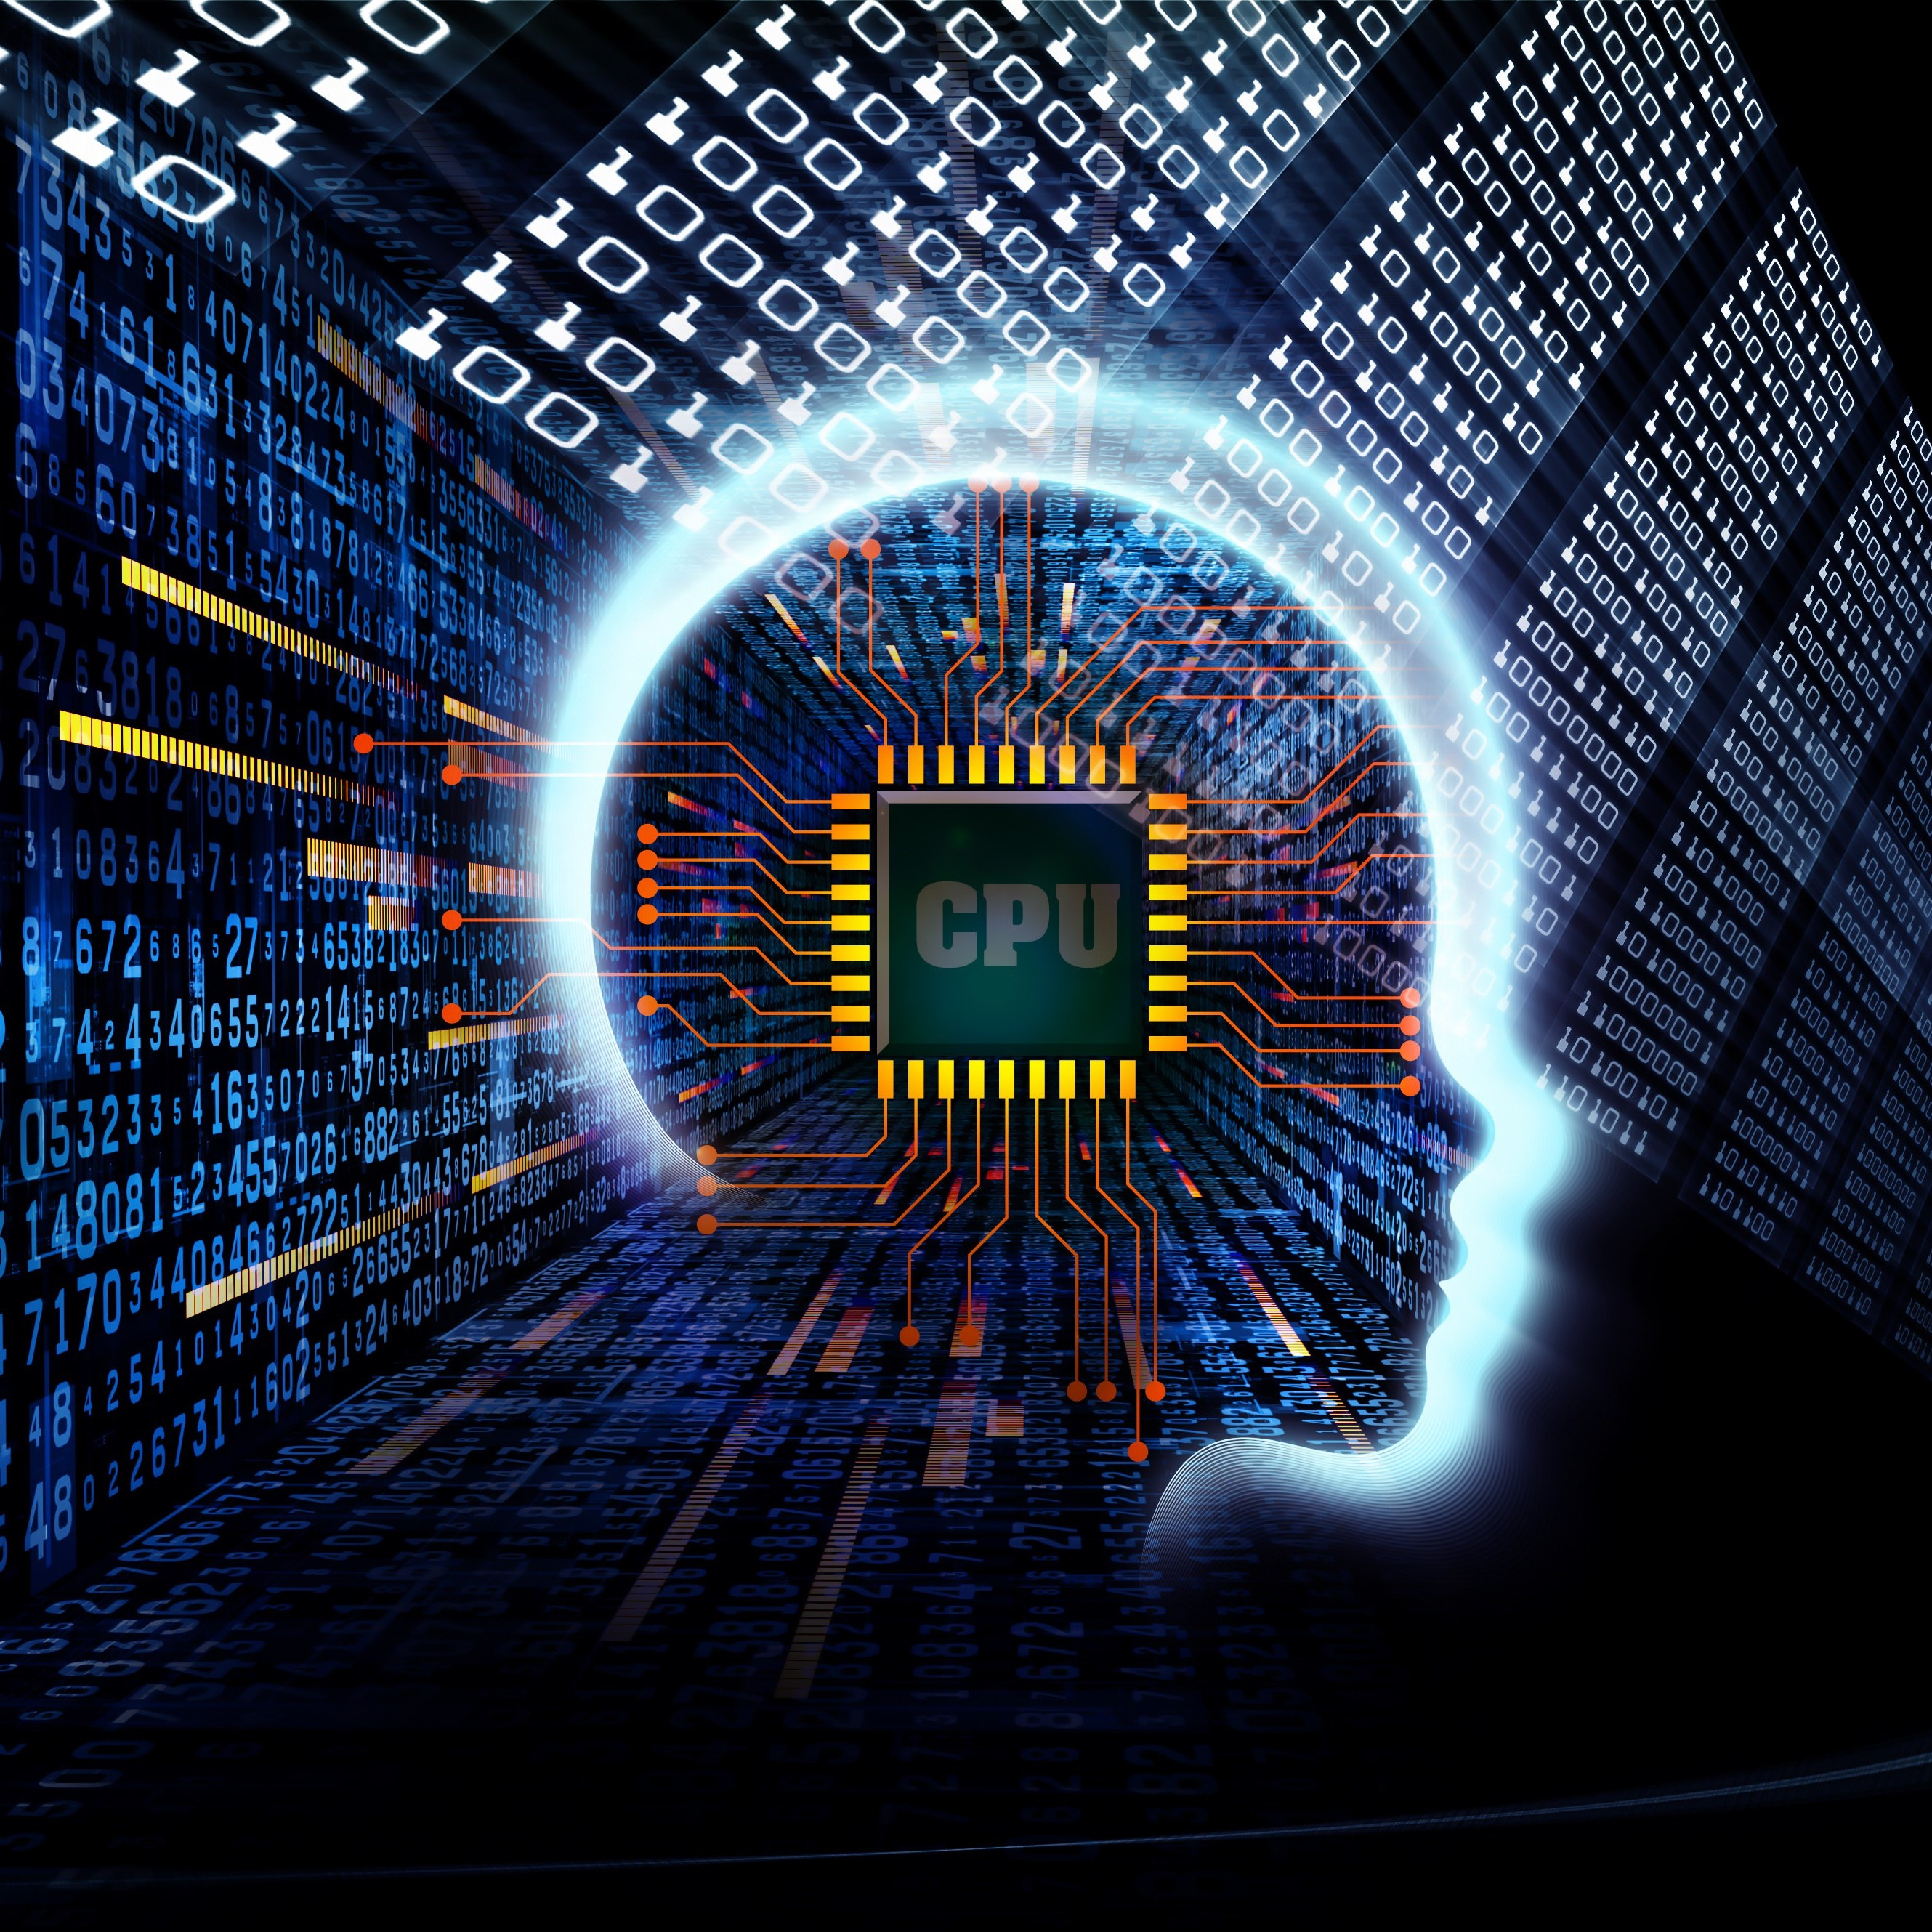
\includegraphics[width=\paperwidth]{capa}};
\draw (8,-22) node [fill=blue!30!white,fill opacity=0.6,text opacity=1,inner sep=1cm]{\Huge\centering\bfseries\sffamily\parbox[c][][t]{\paperwidth}{\centering Assembly na Prática\\[15pt] % Titulo
{\Large Versão 1.0}\\[20pt] % Subtitulo
{\huge Fernando Anselmo}}}; % Nome
\end{tikzpicture}
\vfill
\endgroup

%------------------------------------------------------------------------------------
%	COPYRIGHT PAGE
%------------------------------------------------------------------------------------
\newpage
~\vfill
\thispagestyle{empty}

\noindent Copyright \copyright\ 2021 Fernando Anselmo% Copyright

\noindent \textsc{Publicação Independente} % Publicado por

\noindent \url{http:\\fernandoanselmo.orgfree.com} % URL

\noindent \\ É permitido a total distribuição, cópia e compartilhamento deste arquivo, desde que se preserve os seguintes direitos, conforme a licença da Creative Commons 3.0. Qualquer marca utilizada aqui correspondem aos seus respectivos direitos de marca são reservados. Logos, ícones e outros itens inseridos nesta obra, são da responsabilidade de seus proprietários e foram utilizadas somente como característica informativa. Não possuo qualquer intenção na apropriação da autoria relativo a nenhum artigo de terceiros. Caso não tenha citado a fonte correta de algum texto que coloquei em qualquer seção, basta me enviar um e-mail que farei as devidas retratações, algumas partes podem ter sido cópias (ou baseadas na ideia) de artigos que li na Internet e que me ajudaram a esclarecer muitas dúvidas, considere este como um documento de pesquisa que resolvi compartilhar para ajudar os outros usuários e não é minha intenção tomar crédito de terceiros. % License information

%------------------------------------------------------------------------------------
%	SUMARIO
%------------------------------------------------------------------------------------

% Para nao usar imagem nos capitulos
% \usechapterimagefalse 

\chapterimage{header01.jpg} % Imagem
\pagestyle{empty} % Sem Cabecalho
\tableofcontents % Mostra a tabela de conteudo
\cleardoublepage % Forca que a primeira pagina seja iniciada em um numero impar
\pagestyle{fancy} % Volta a imprimir o Cabecalho
\clearpage % Forca que a primeira pagina seja iniciada em um numero impar

%------------------------------------------------------------------------------------
%	PARTES
%------------------------------------------------------------------------------------

% \part{Parte Um - O Básico}
%------------------------------------------------------------------------------------
%	CHAPTER 1
%------------------------------------------------------------------------------------
\chapterimage{headMontagem.png}
\chapter{Entendimento Geral}

\begin{remark}
"Um bom programador não se define pelas ferramentas que usa, mas pelo que aprende ao dominá-las — como o Pascal ensina." (\textit{Alan Perlis}, primeiro vencedor do prêmio Turing.) 
\end{remark}

\section{Do que trata esse livro?}\index{Entendimento Geral}
\textbf{Pascal} foi criada em 1970 pelo cientista da computação suíço \textbf{Niklaus Wirth}. Seu objetivo principal foi desenvolver uma linguagem que fosse eficiente, fácil de aprender e que promovesse boas práticas de programação, como por exemplo, o ensino da Lógica de Programação. Inspirada por linguagens anteriores como \textbf{ALGOL}, \textbf{Pascal} foi projetada para ensinar conceitos fundamentais de programação estruturada e desenvolvimento de software, sendo amplamente adotada em ambientes acadêmicos durante as décadas de 1970 e 1980.

O nome da linguagem é uma homenagem ao matemático e filósofo francês \textbf{Blaise Pascal}, conhecido por suas contribuições à matemática e pela invenção de uma das primeiras calculadoras mecânicas, como a \textit{Pascalina}\footnote{A Pascalina foi uma das primeiras calculadoras mecânicas da história, criada pelo matemático, físico e filósofo francês \textbf{Blaise Pascal} em 1642, quando ele tinha apenas 19 anos. Foi projetada para ajudar seu pai, \textbf{Étienne Pascal}, que trabalhava como coletor de impostos e precisava realizar muitos cálculos repetitivos. A invenção marcou um marco significativo no desenvolvimento das máquinas de cálculo.}. A linguagem Pascal trouxe inovações importantes, como a ênfase em estruturas de controle claras (condicionais e laços) e na organização modular de programas, o que ajudou os desenvolvedores a criar código legível e fácil de manter.

Embora inicialmente projetada para ensinar, a linguagem logo encontrou aplicações práticas na indústria. Versões como \textbf{Turbo Pascal}, lançada pela \textbf{Borland} na década de 1980, tornaram-se extremamente populares devido à sua rapidez, facilidade de uso e baixo custo. \textbf{Turbo Pascal} oferecia um ambiente de desenvolvimento integrado (IDE) que permitia aos programadores escrever, compilar e executar programas de forma eficiente, algo revolucionário para a época.

Ao longo do tempo, \textbf{Pascal} evoluiu e deu origem a variantes como \textbf{Object Pascal}, que introduziu conceitos de programação orientada a objetos e serviu de base para o desenvolvimento de ferramentas como o \textbf{Delphi}, um ambiente robusto para criar aplicações gráficas para o sistema \textbf{Windows} (na época seu único concorrente era o Visual Basic da própria \textbf{Microsoft}).

Embora Pascal tenha perdido popularidade com o surgimento de linguagens mais modernas derivadas do \textbf{C}, sua influência persiste. Muitos programadores veteranos aprenderam conceitos fundamentais de computação usando o \textbf{Pascal}, e sua ênfase em clareza e estrutura continua sendo uma lição valiosa para a programação até hoje.

\section{Quais são as vantagens de se aprender Pascal atualmente?}\index{Entendimento Geral}
Aprender a linguagem Pascal hoje pode oferecer algumas vantagens, dependendo do contexto e do objetivo de aprendizado. Aqui estão algumas delas:
\begin{itemize}
	\item \textbf{Fundamentos de programação}: é uma linguagem muito boa para aprender os conceitos básicos de programação, como variáveis, estruturas de controle, funções e tipos de dados. Sua sintaxe simples e clara ajuda a focar no raciocínio lógico sem sobrecarregar o aluno com complexidade.
	\item \textbf{Educação}: universidades e escolas a usam como linguagem introdutória em cursos de ciência da computação no passado. Embora outras linguagens tenham substituído em muitos lugares, a base sólida que Pascal oferece ainda é valiosa em cursos que ensinam os fundamentos da programação.
	\item \textbf{Histórico e legado}: o conhecimento pode ser útil caso seja necessário trabalhar em projetos legados ou sistemas que ainda utilizam essa linguagem. Alguns softwares mais antigos, especialmente em áreas como automação industrial e sistemas embarcados, são escritos em Pascal e exigem conhecimento nesta (seja para manutenção ou mesmo migração).
	\item \textbf{Clareza e estrutura}: \textbf{Pascal} foi projetada para ser fácil de entender e ensinar. Sua sintaxe é bastante rígida, o que pode ajudar a evitar maus hábitos na programação.
	\item \textbf{Portabilidade}: compiladores modernos para Pascal (como \textbf{Free Pascal}) que permitem rodar o código em diferentes plataformas. Isso pode ser interessante para quem deseja experimentar linguagens de baixo nível ou desenvolver software que precise ser altamente eficiente.
	\item \textbf{Desenvolvimento de algoritmos}: sendo uma linguagem estruturada, é muito boa para o desenvolvimento e análise de algoritmos, sem a complexidade de recursos modernos visto em outras linguagens.
\end{itemize}
Essas vantagens tornam o COBOL uma escolha interessante para quem deseja trabalhar em áreas que envolvem sistemas legados e infraestrutura crítica, permite abrir portas para um conjunto especializado de habilidades que ainda tem grande valor no mercado de trabalho.

\section{Montagem do Ambiente}\index{Entendimento Geral}
Podemos montar nosso ambiente de desenvolvimento sobre diversos sistemas operacionais, oferecendo flexibilidade na escolha da plataforma ideal para o projeto. Neste livro, é utilizado o Ubuntu 24.10, uma das distribuições Linux mais populares e acessíveis, conhecida por sua estabilidade, segurança e suporte a uma vasta gama de ferramentas de desenvolvimento.

O uso de software livre é uma das principais vantagens deste ambiente, pois todos os programas e bibliotecas necessárias para o desenvolvimento estarão disponíveis gratuitamente, sem custos adicionais. Isso inclui editores de código, ferramentas de automação e depuração, que são perfeitamente adequados para projetos profissionais. Além disso, o hardware necessário é simples: um computador (que provavelmente já possui), sem a necessidade de investimentos adicionais em equipamentos especializados. Com isso, podemos configurar um ambiente de desenvolvimento poderoso e eficiente, aproveitando ao máximo os recursos do Ubuntu e dos softwares livres, sem comprometer o orçamento.

Iremos utilizar o \textbf{Free Pascal}, assim na tela de terminal usamos o seguinte comando: \\
\codigo{\$ sudo apt install fpc}

Necessitamos de um editor de códigos, recomendo o Visual Studio Code, não apenas pela leveza pois, dentre todos os editores é o que melhor se adapta a linguagem Pascal através dos plugins. \\
\codigo{\$ snap install code}

Criamos uma pasta para manter nossos códigos arrumados: \\
\codigo{\$ mkdir pascalProjects}

Entramos nessa pasta: \\
\codigo{\$ cd pascalProjects}

E no editor: \\
\codigo{\$ code .}

Na seção \textbf{Extensões}, instalamos o seguinte plugin:
\begin{itemize}
	\item FreePascal Toolkit - Fornecedor: coolchyni
\end{itemize}

E agora estamos prontos para criarmos e executarmos nosso primeiro programa em máquinas atuais na linguagem Pascal.

\section{Mais sobre a Pascalina}\index{Entendimento Geral}
As pessoas confundem a \textbf{Pascalina} (calculadora criada por \textbf{Blaise Pascal}) com a Máquina Diferencial (1822) de \textbf{Charles Babbage}, que era também um dispositivo mecânico para calcular e imprimir tabelas matemáticas, como as de logaritmos.

\begin{figure}[H]
	\centering
	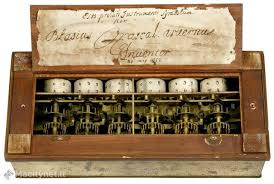
\includegraphics[width=0.5\textwidth]{cap01/pascalina.jpeg}
	\caption{Pascalina}
\end{figure}

A \textbf{Pascalina} era uma máquina baseada em engrenagens que podia realizar operações básicas de adição e subtração. Seu mecanismo utilizava rodas dentadas numeradas de 0 a 9, conectadas de forma que, ao girar uma roda, os números fossem ajustados automaticamente. O sistema implementava a ideia de "transbordo" (ou carry), em que, ao ultrapassar o valor 9, uma roda fazia a próxima avançar, semelhante ao funcionamento dos odômetros. 

Embora a Pascalina fosse uma tecnologia revolucionária para a época, ela não teve ampla adoção devido ao seu alto custo de fabricação e à complexidade de operação. Ainda assim, a máquina é considerada um marco na história da computação, pois foi uma das primeiras tentativas de automatizar cálculos, reduzindo o esforço humano e os erros associados ao trabalho manual. Atualmente está preservada em museus e representada em reproduções, e continua sendo um símbolo da engenhosidade humana e um precursor das modernas calculadoras e computadores.

Se deseja conhecer mais sobre esse fantástico projeto, assista o vídeo do Canal "What Will Makes" \url{https://www.youtube.com/watch?v=E0pJST5mL3A&t=2s}, onde um jovem engenheiro mostra passo a passo da execução de um projeto similar.

\clearpage
%------------------------------------------------------------------------------------
%	CHAPTER 2
%------------------------------------------------------------------------------------
\chapterimage{headMontagem.png}
\chapter{Passos Iniciais}

\begin{remark}
	"Aprender uma linguagem como Pascal é mais do que aprender a programar; é aprender a pensar logicamente." (\textit{Donald Knuth}, cientista da computação.) 
\end{remark}

\section{Hello World}\index{Passos Iniciais}
É tradição no mundo da programação que devemos começar com o programa "Hello World" quando estamos iniciando o estudo de uma nova linguagem, e quem sou eu para quebrar essa tradição, assim, aqui está o famoso "Hello World" em Pascal:
\begin{lstlisting}[]
program hello;

begin
  WriteLn('Hello World!');
end.
\end{lstlisting}

Chega a ser extremamente simples comparando com outras linguagens, o programa sempre inicia com a palavra reservada \textbf{program} e seguida o nome deste, finalizamos a instrução com um ";" (ponto e vírgula). O corpo principal do programa está entre na palavra reservada \textbf{begin} e seu término \textbf{end} que dessa vez deve ser finalizado com um "." (ponto final). E agora temos o comando, ou função se preferir, \textbf{WriteLn} que mostra algo na tela, neste caso o literal 'Hello World!', e uma observação muito importante, não utilizamos ASPAS DUPLAS (como os acostumados das linguagens derivadas de \textbf{C}) mas ASPAS SIMPLES para indicar as literais.

Salvamos este programa com o nome \textit{Hello.pas} (o nome não precisa ser o mesmo da cláusula \textbf{program}), e em seguida devemos compilar com o comando: \\
\codigo{\$ fpc Hello.pas}

Nesse momento aconteceu a magia pois o nosso programa foi transformado em um executável do Linux e basta apenas o comando: \\
\codigo{\$ ./Hello}

\section{Obtendo valores}\index{Passos Iniciais}
Agora que já agradamos aos deuses da programação, vamos tentar algo mais elaborado, como obter a entrada de duas variáveis numéricas e proceder cálculos aritméticos.

\begin{lstlisting}[]
program calculadora;
var 
  a,b: integer;

begin
  write('Informe o valor de a: ');
  read(a);
  write('Informe o valor de b: ');
  read(b);
  writeln('A soma é: ', a+b);
  writeln('A subtração é: ', a-b);
  writeln('A divisão é: ', a/b);
  writeln('A multiplicação é: ', a*b);
end.
\end{lstlisting}

Na linguagem Pascal não se importa se escrevemos as funções em letras maiúsculas ou minúsculas (desde que escritas corretamente), assim use a forma que preferir para estas.

Após a definição do programa, temos a palavra chave \textbf{var} que define duas variáveis inteiras \textbf{a} e \textbf{b}. Primeiro solicitamos o valor da primeira, a diferença entre as funções \textbf{write()} e \textbf{writeln()} e que a primeira escreve o valor e para o cursos no mesmo lugar enquanto que a segunda salta para a próxima linha. A função \textbf{read()} aguarda até que o usuário informe um valor e pressione a tecla ENTER e coloca o valor na variável selecionada.

Neste ponto podemos ter um erro no programa, note que nossa variável foi definida com um valor inteiro, caso o usuário informe algo diferente recebemos um \textbf{Runtime error}.

Considerando que dois valores foram informados corretamente, mostramos a soma (+), subtração (-), divisão (/) e multiplicação (*) desses, utilizamos a "," (virgula) para separar o literal do resultado.

Salvamos este programa com o nome \textit{Hello.pas} (o nome não precisa ser o mesmo da cláusula \textbf{program}), e em seguida devemos compilar com o comando: \\
\codigo{\$ fpc Calculadora.pas}

Nesse momento aconteceu a magia pois o nosso programa foi transformado em um executável do Linux e basta apenas o comando: \\
\codigo{\$ ./Calculadora}

\section{Fórmula de Bháskara}\index{Passos Iniciais}
Esse programa resolve uma equação do segundo grau com a utilização da \textbf{Fórmula de Bhaskara}.
\begin{lstlisting}[]
program bhaskara;
var
  a, b, c: integer;
var
  delta: real;

begin
  write('Informe o valor da raiz a: ');
  read(a);
  write('Informe o valor da raiz b: ');
  read(b);
  write('Informe o valor da raiz c: ');
  read(c);

  delta := (b*b) - (4*a*c);

  writeln('Para a função ', a, 'x^2 + ', b, 'x + ', c, ' temos:');
  if delta < 0 then
    writeln('Não existem raízes reais.')
  else if delta = 0 then
    writeln('Existe apenas uma raiz real: ', -b / (2 * a) :5:2)
  else
    begin
      writeln('Delta: ', delta:5:2);
      writeln('x' : ', (-b + sqrt(delta)) / (2*a) :5:2);
      writeln('x'' : ', (-b - sqrt(delta)) / (2*a) :5:2);
    end;
end.	
\end{lstlisting}

Começamos o programa com a definição de dois grupos de variáveis:  \vspace{-1em}
\begin{itemize}
	\item a, b, c: São os coeficientes da equação do segundo grau $ax^2 + bx + c = 0$. Foram declarados como inteiros (integer).
	\item delta: É valor decimal (real). O delta é a parte da fórmula de Bháskara que determina se existem raízes reais.
\end{itemize}

A primeira parte, do programa propriamente dito, obtém os valores de \textbf{a}, \textbf{b} e \textbf{c}. Calculamos o valor de Delta, com base na seguinte fórmula:
\[
\Delta = b^2 - 4ac
\]
A variável \textbf{delta} (uma variável auxiliar) armazena esse cálculo. Uma vez que temos esse valor, podemos julgá-lo para verificar se a equação tem soluções reais: \vspace{-1em}
\begin{itemize}
	\item Se $\delta < 0$, não existem raízes reais (não há solução no conjunto dos números reais).
	\item Se $\delta = 0$, há uma única raiz real, pois a fórmula se reduz $a - b / 2a$.
\end{itemize}

As raízes são calculadas com a fórmula:
\[
  x = \frac{-b \pm \sqrt{\Delta}}{2a}
\]
Salvamos este programa com o nome \textit{Equacao.pas}, e em seguida devemos compilar com o comando: \\
\codigo{\$ fpc Equacao.pas}

E executamos com o comando: \\
\codigo{\$ ./Equacao}

O programa funciona perfeitamente porém não é assim que normalmente usamos uma linguagem estruturada, pois dessa forma não estaremos facilitando a manutenção. Vamos utilizar 2 componentes em Pascal. \vspace{-2em}
\begin{enumerate}
	\item \textbf{Função (function)} - Uma função retorna um valor. Ou seja, calcula algo e retorna um determinado resultado.
	\item \textbf{Procedimento (procedure)} - Um procedimento não retorna valores diretamente. Utilizado para executar ações, como exibir mensagens ou modificar variáveis.
\end{enumerate}

Estrutura de uma função:
\begin{lstlisting}[]
function NomeDaFuncao(parametros): TipoDeRetorno;
begin
  NomeDaFuncao := valor;  { Retorna um valor }
end;
\end{lstlisting}

Estrutura de um procedimento:
\begin{lstlisting}[]
procedure NomeDoProcedimento(parametros);
begin
  { Faz algo, mas não retorna nada }
end;	
\end{lstlisting}

Sabendo disso, agora podemos reescrever o mesmo programa para:
\begin{lstlisting}[]
program bhaskara;

uses math;  { Para usar a função sqrt() }

{ Função para ler um número inteiro com uma mensagem personalizada }
function lerNumero(msg: string): integer;
begin
  write(msg);
  readln(lerNumero);
end;

{ Função para calcular Delta }
function calcularDelta(a, b, c: integer): real;
begin
  calcularDelta := (b * b) - (4 * a * c);
end;

{ Procedimento para calcular e exibir as raízes, se existirem }
procedure calcularRaizes(a, b: integer; delta: real);
var
  raiz1, raiz2: real;
begin
  if delta < 0 then
    writeln('Não existem raízes reais.')
  else if delta = 0 then
    writeln('Existe apenas uma raiz real: ', -b / (2 * a) :5:2)
  else
    begin
      raiz1 := (-b + sqrt(delta)) / (2 * a);
      raiz2 := (-b - sqrt(delta)) / (2 * a);
      writeln('Delta: ', delta:5:2);
      writeln('x' : ', raiz1:5:2);
      writeln('x'' : ', raiz2:5:2);
    end;
end;

{ Procedimento para ler os coeficientes da equação }
procedure lerCoeficientes(var a, b, c: integer);
begin
  a := lerNumero('Informe o valor de a: ');
  b := lerNumero('Informe o valor de b: ');
  c := lerNumero('Informe o valor de c: ');
end;

{ Programa principal }
var
  a, b, c: integer;
  delta: real;
begin
  lerCoeficientes(a, b, c);
  delta := calcularDelta(a, b, c);
  writeln('Para a função ', a, 'x^2 + ', b, 'x + ', c, ' temos:');
  calcularRaizes(a, b, delta);
end.
\end{lstlisting}

Com isso posto, apesar do programa ter crescido muito, observamos uma melhor legibilidade pois o código principal ficou menor e mais fácil de entender. Além disso podemos reusar várias funções ou procedimentos em diversos outros programas.

\clearpage
%------------------------------------------------------------------------------------
%	CHAPTER 3
%------------------------------------------------------------------------------------
\chapterimage{headSpark.png}
\chapter{Aprofundando no Spark}

\begin{remark}
"Uma única centelha de criatividade pode desencadear uma revolução tecnológica e transformar o mundo." (Elon Musk) 
\end{remark}

\section{Melhora dos Dados Estatísticos}\index{Aprofundando no Spark}
\textbf{Ming Chen} e \textbf{Wenqiang Feng} escreveram um excelente método que se compara bem ao método describe() da biblioteca Pandas (com algumas vantagens), sendo assim, vamos aplicá-la. Criamos um novo notebook e em uma célula a conexão com o Spark:
\begin{lstlisting}[]
from pyspark.sql import SparkSession

spark = SparkSession.\
        builder.\
        appName("pyspark-notebook").\
        master("spark://spark-master:7077").\
        config("spark.executor.memory", "512m").\
        getOrCreate()
\end{lstlisting}

Em seguida criamos um Dataframe:
\begin{lstlisting}[]
df_pyspark = spark.read.csv('dados2.csv', header=True, inferSchema=True)
df_pyspark.show()
\end{lstlisting}

Lembre-se que o arquivo se encontra disponível no GitHub, usamos o método describe nativo:
\begin{lstlisting}[]
df_pyspark.describe().show()
\end{lstlisting}

E temos o seguinte resultado:
 \vspace{-1.5em}
\begin{verbatim}
+-------+---------+------------------+------------------+
|summary|     Nome|             Idade|       Experiencia|
+-------+---------+------------------+------------------+
|  count|       54|                54|                54|
|   mean|     null| 44.96296296296296|107.57407407407408|
| stddev|     null|15.026973185930618| 86.78679185044531|
|    min|    Alice|                18|                 0|
|    max|Valentina|                73|               444|
+-------+---------+------------------+------------------+
\end{verbatim}

Agora precisamos usar o Pandas, apenas para organizar melhor a informação:
\begin{lstlisting}[]
!pip install pandas
\end{lstlisting}

Uma vez instalado, podemos realizar as importações necessárias para execução do método:
\begin{lstlisting}[]
import numpy as np
import pandas as pd
\end{lstlisting}

E criar o método:
\begin{lstlisting}[]
def describe_pd(df_in, columns, deciles=False):
    if deciles:
        percentiles = np.array(range(0, 110, 10))
    else:
        percentiles = [25, 50, 75]
    percs = np.transpose([np.percentile(df_in.select(x).collect(),percentiles) for x in columns])
    percs = pd.DataFrame(percs, columns=columns)
    percs['summary'] = [str(p) + '%' for p in percentiles]
    spark_describe = df_in.describe().toPandas()
    new_df = pd.concat([spark_describe, percs],ignore_index=True)
    new_df = new_df.round(2)
    return new_df[['summary'] + columns]
\end{lstlisting}

Esse método pode ser trabalhado tanto com deciles quanto os percentis, para usar os deciles basta usar o parâmetro "deciles=True", por padrão a saída é dada em percentis, porém só podemos usar as colunas numéricas, do seguinte modo:
\begin{lstlisting}[]
describe_pd(df_pyspark, ['Idade', 'Experiencia'])
\end{lstlisting}

E temos como resultado:
\begin{figure}[H]
	\centering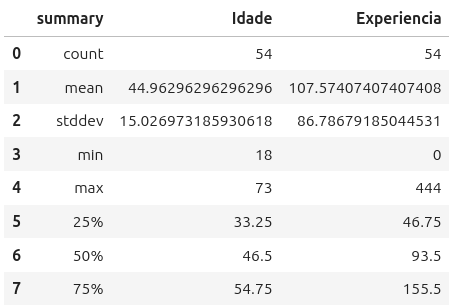
\includegraphics[scale=0.45]{cap03/SaidaDescribe}
	\caption{Saída do método describe\_pd()}
\end{figure}

E deste modo obtemos um visual bem mais agradável.

\section{Assimetria e Curtose}\index{Aprofundando no Spark}

Na probabilidade, \textbf{assimetria} (ou \textit{skewness} em inglês) é uma medida de assimetria da distribuição de probabilidade em uma variável aleatória com valores reais em relação à sua média. O valor de assimetria pode ser positivo, negativo ou indefinido. Para uma distribuição unimodal, uma assimetria negativa indica comumente que a cauda está do lado esquerdo da distribuição, enquanto uma assimetria positiva indica que a cauda está do lado direito.

Já a palavra, \textbf{curtose} (ou \textit{kurtosis} em inglês, também escrito como "kyrtos" ou "kurtos", significando "curvado, arqueado") é uma medida de "caudalidade" da distribuição de probabilidade em uma variável aleatória com valores reais. De maneira similar ao conceito de assimetria, a curtose é um descritor da forma em uma distribuição de probabilidade e, assim como para a assimetria, existem diferentes maneiras de quantificá-la para uma distribuição teórica e métodos correspondentes para estimá-la a partir da amostra de uma população.

Importamos as bibliotecas necessárias:
\begin{lstlisting}[]
from pyspark.sql.functions import col, skewness, kurtosis
\end{lstlisting}

E executamos os métodos para a variável idade:
\begin{lstlisting}[]
df_pyspark.select(skewness(df_pyspark.Idade),kurtosis(df_pyspark.Idade)).show()
\end{lstlisting}

E temos o seguinte resultado:
 \vspace{-1.5em}
\begin{verbatim}
+-------------------+-------------------+
|    skewness(Idade)|    kurtosis(Idade)|
+-------------------+-------------------+
|0.08635507023568641|-0.9555352263232475|
+-------------------+-------------------+
\end{verbatim}

Uma assimetria positiva indica que a cauda direita é mais longa, se fosse uma assimetria negativa a cauda esquerda seria mais longa, em relação a um centro típico dos dados. Vejamos isso graficamente, porém precisamos instalar a biblioteca SeaBorn:
\begin{lstlisting}[]
!pip install seaborn
\end{lstlisting}

Uma vez instalada, podemos importar as bibliotecas necessárias:
\begin{lstlisting}[]
\textbf{import seaborn as sns
import matplotlib.pyplot as plt
%matplotlib inline}
\end{lstlisting}

Obter os valores que serão mostrados:
\begin{lstlisting}[]
coluna_selecionada = df_pyspark.select("Idade")
x = coluna_selecionada.rdd.flatMap(lambda x: x).collect()
\end{lstlisting}

E mostrar o gráfico:
\begin{lstlisting}[]
plt.figure(figsize=(8,4))
sns.histplot(x, kde=True)
plt.xlabel('Idade')
plt.ylabel('Quantidade')
plt.show()
\end{lstlisting}

E temos como resultado:
\begin{figure}[H]
	\centering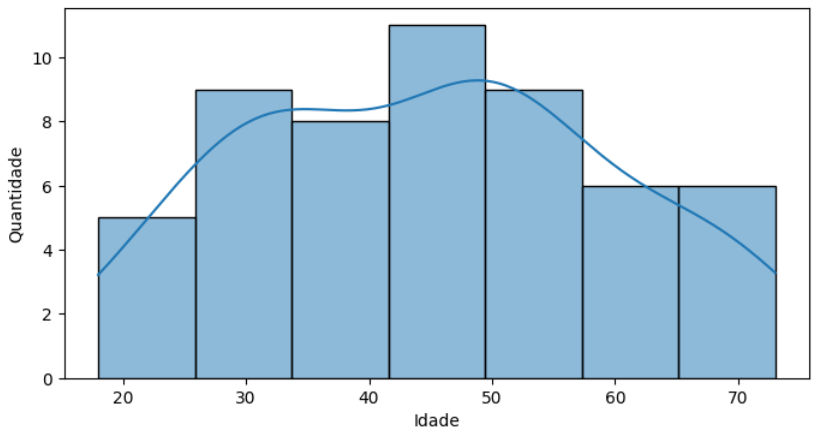
\includegraphics[scale=0.45]{cap03/GraficoDistribuicao}
	\caption{Gráfico da Distribuição por Idade}
\end{figure}

\section{Métodos Estatísticos com RDD}\index{Aprofundando no Spark}
Objetos RDD são interessantes quando desejamos informações básicas estatísticas, nesta seção veremos uma série de exemplos, inicialmente criamos um novo notebook e iniciamos a seção do Spark neste:
\begin{lstlisting}[]
from pyspark.sql import SparkSession

spark = SparkSession.\
        builder.\
        appName("pyspark-notebook").\
        master("spark://spark-master:7077").\
        config("spark.executor.memory", "512m").\
        getOrCreate()
        
sc = spark.sparkContext        
\end{lstlisting}

Criamos nossos dados através da paralelização de uma lista de valores:
\begin{lstlisting}[]
numsRdd = sc.parallelize((2, 4, 6, 8, 3, 2, 8, 1, 4, 7))
\end{lstlisting}

A média aritmética desses valores:
\begin{lstlisting}[]
numsRdd.mean()
\end{lstlisting}

E obtemos o valor: \\
{\ttfamily 4.5}

A quantidade de elementos (ou amostras):
\begin{lstlisting}[]
numsRdd.count()
\end{lstlisting}

E obtemos o valor: \\
{\ttfamily 10}

Quantidade de cada um dos valores:
\begin{lstlisting}[]
numsRdd.countByValue()
\end{lstlisting}

E obtemos o valor: \\
{\ttfamily defaultdict(int, \{2: 2, 4: 2, 6: 1, 8: 2, 3: 1, 1: 1, 7: 1\})}

O primeiro valor da lista:
\begin{lstlisting}[]
numsRdd.first()
\end{lstlisting}

E obtemos o valor: \\
{\ttfamily 2}

O maior e menor valor da lista
\begin{lstlisting}[]
print(numsRdd.max(), numsRdd.min())
\end{lstlisting}

E obtemos os valores: \\
{\ttfamily 8 1}

Desvio padrão:
\begin{lstlisting}[]
numsRdd.stdev()
\end{lstlisting}

E obtemos o valor: \\
{\ttfamily 2.4596747752497685}

A soma total dos valores:
\begin{lstlisting}[]
numsRdd.sum()
\end{lstlisting}

E obtemos o valor: \\
{\ttfamily 45}

Também podemos usar o método de agregação \textit{fold()} que reúne os elementos do RDD através um valor neutro especificado (valor zero) e um operador binário associativo. Primeiro agrega os elementos em cada partição do RDD e, em seguida, agrega os resultados de cada partição:
\begin{lstlisting}[]
# Soma de todos os elementos do RDD
soma = numbersRdd.fold(0, lambda x, y: x + y)

# Produto de todos os elementos do RDD
produto = numbersRdd.fold(1, lambda x, y: x * y)
print(soma, produto)
\end{lstlisting}

E obtemos os valores: \\
{\ttfamily 45 516096}

Neste exemplo, o método fold() recebe dois argumentos: o primeiro é o valor inicial (0 para a soma e 1 para o produto) e o segundo é a função lambda que combina os elementos do RDD (soma ou multiplicação) de acordo com a operação desejada.

Porém é mais eficiente utilizarmos o método reduce() que agrega os elementos do RDD usando um operador binário associativo e comutativo fornecido. É semelhante ao método fold(); no entanto, não requer um valor neutro:
\begin{lstlisting}[]
# Soma de todos os elementos do RDD
soma = numbersRdd.reduce(lambda x, y: x + y)

# Produto de todos os elementos do RDD
produto = numbersRdd.reduce(lambda x, y: x * y)
print(soma, produto)
\end{lstlisting}

E teremos o mesmo resultado, a diferença é que o método reduce() recebe somente a função lambda com dois argumentos (x e y), representando dois elementos do RDD que serão combinados para calcular o resultado final. 

E a variância:
\begin{lstlisting}[]
numsRdd.variance()
\end{lstlisting}

E obtemos o valor: \\
{\ttfamily 6.05}

Não esquecer de encerrar a seção:
\begin{lstlisting}[]
spark.sparkContext.stop()
\end{lstlisting}

\clearpage

% 
\appendix
\chapter{Considerações Finais}
\begin{remark}
Nenhum computador tem consciência do que faz. 
Mas, na maior parte do tempo, nós também não. (Marvin Minsky)
\end{remark}

\section{Sobre o Autor}
Especialista com forte experiência em Java e Python, Banco de Dados Oracle, PostgreSQL e MS SQL Server. Escolhido como Java Champion desde Dezembro/2006 e Coordenador do DFJUG. Experiência em JBoss e diversos frameworks de mercado e na interpretação das tecnologias para sistemas e aplicativos. Programação de acordo com as especificações, normas, padrões e prazos estabelecidos. Disposição para oferecer apoio e suporte técnico a outros profissionais, autor de 17 livros e diversos artigos em revistas especializadas, palestrante em diversos seminários sobre tecnologia. Atualmente ocupa o cargo de Analista de Sistemas na Bancorbras.
\begin{itemize}
 \item Perfil no Linkedin: \url{https://www.linkedin.com/in/fernando-anselmo-bb423623/}
 \item Site Pessoal: \url{http://fernandoanselmo.orgfree.com} 
\end{itemize}

\clearpage
%------------------------------------------------------------------------------------
%	FINAL PAGE
%------------------------------------------------------------------------------------
\begingroup
\thispagestyle{empty}
\begin{tikzpicture}[remember picture,overlay]
\node[inner sep=0pt] (background) at (current page.center) {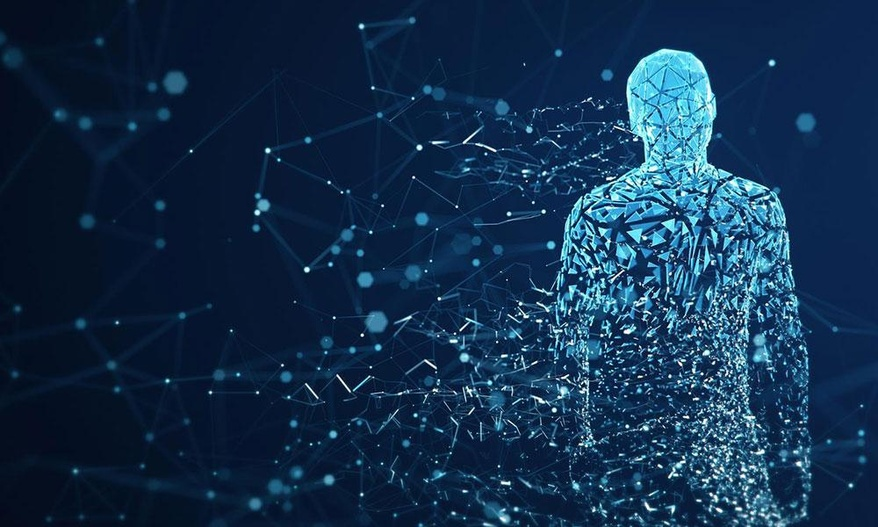
\includegraphics[width=\paperwidth]{fundo}};
\draw (8,-2) node [fill=blue!30!white,fill opacity=0.6,text opacity=1,inner sep=1cm]{\Huge\centering\bfseries\sffamily\parbox[c][][t]{\paperwidth}{\centering Assembly na Prática\\[15pt] % Titulo
{\Large ESTE LIVRO PODE E DEVE SER DISTRIBUÍDO LIVREMENTE}\\[20pt] % Subtitulo
{\huge Fernando Anselmo}}}; % Nome
\end{tikzpicture}
\vfill
\endgroup

%------------------------------------------------------------------------------------
%	INDEX
%------------------------------------------------------------------------------------
% \cleardoublepage
% \phantomsection
% \setlength{\columnsep}{0.75cm}
% \addcontentsline{toc}{chapter}{\textcolor{ocre}{Index}}
% \printindex

%------------------------------------------------------------------------------------
\end{document}
